\documentclass[11pt,a4paper]{article}
\usepackage[utf8]{inputenc}
\usepackage[T1]{fontenc}
\usepackage{amsmath,amssymb,amsfonts}
\usepackage{graphicx}
\usepackage{booktabs}
\usepackage{multirow}
\usepackage{float}
\usepackage[margin=2.5cm]{geometry}
\usepackage{hyperref}
\usepackage{algorithm}
\usepackage{algpseudocode}
\usepackage{xcolor}
\usepackage{caption}
\usepackage{subcaption}
\usepackage{tikz}
\usetikzlibrary{shapes.geometric, arrows.meta, positioning, calc, shadows}

\title{Methodology for Multi-Task Affective State Recognition Using Gradient Boosting}
\author{}
\date{}

\begin{document}
\maketitle

\section{Methodology}

\begin{figure}[H]
\centering
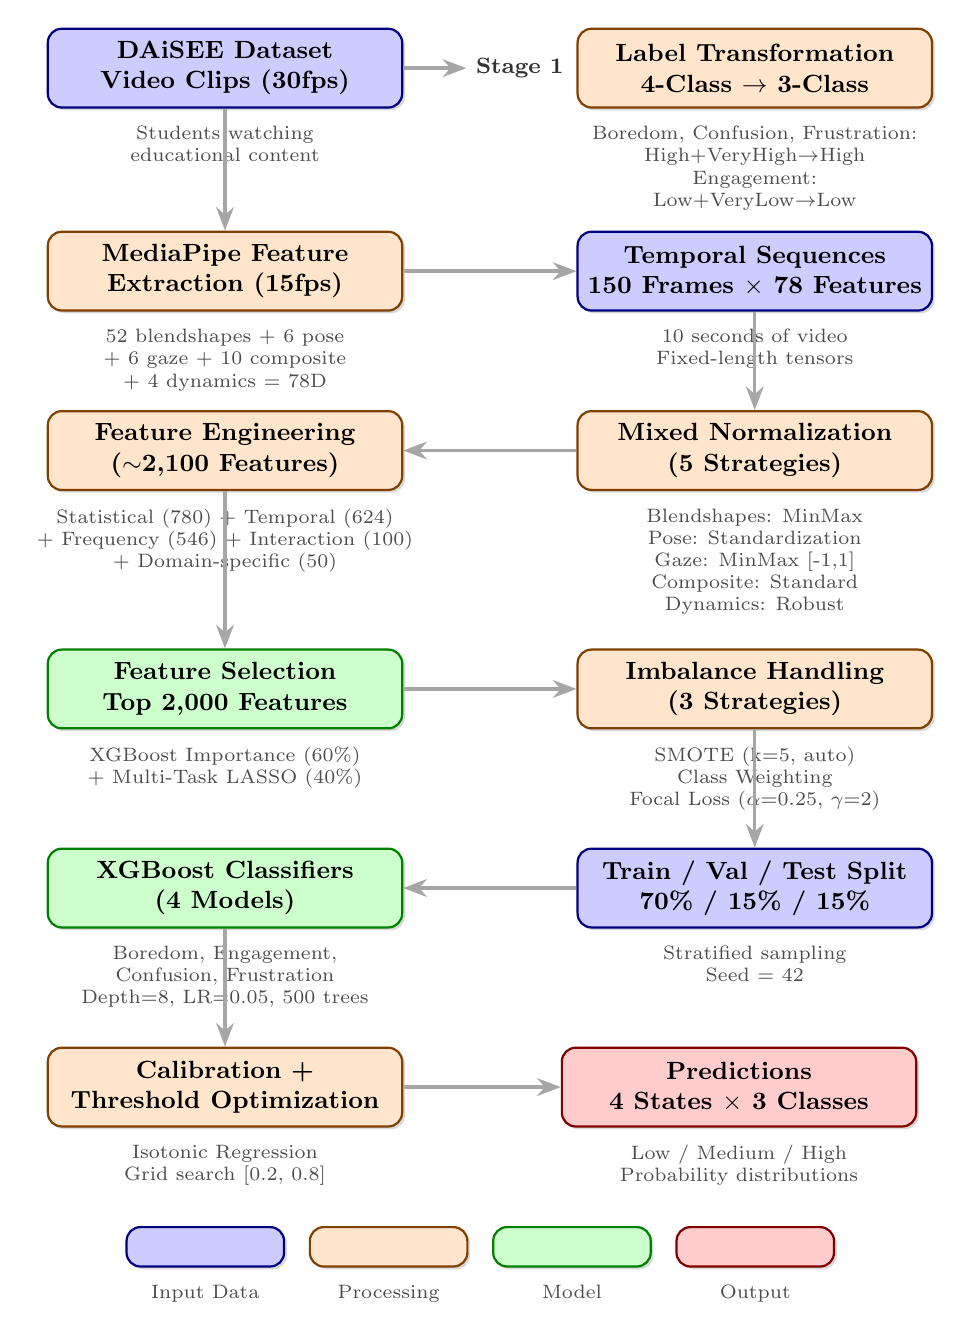
\begin{tikzpicture}[
    node distance=0.8cm and 1.5cm,
    box/.style={
        rectangle, rounded corners=5pt, minimum width=4.5cm, minimum height=1cm,
        text centered, align=center, font=\small\bfseries, drop shadow={shadow xshift=1pt, shadow yshift=-1pt, opacity=0.3}
    },
    data/.style={box, fill=blue!20, draw=blue!50!black, thick},
    process/.style={box, fill=orange!20, draw=orange!50!black, thick},
    model/.style={box, fill=green!20, draw=green!50!black, thick},
    output/.style={box, fill=red!20, draw=red!50!black, thick},
    arrow/.style={-{Stealth[length=3mm]}, line width=1.2pt, draw=gray!70},
    label/.style={font=\scriptsize, text=gray!60!black, align=center},
    stage/.style={font=\footnotesize\bfseries, text=gray!40!black}
]

% Stage 1: Input Data
\node[data] (daisee) {DAiSEE Dataset\\Video Clips (30fps)};
\node[label, below=0.1cm of daisee] {Students watching\\educational content};

% Arrow
\node[stage, right=0.8cm of daisee] {Stage 1};
\draw[arrow] (daisee.east) -- ++(0.8cm,0);

% Stage 2: Label Transformation
\node[process, right=2.2cm of daisee] (labels) {Label Transformation\\4-Class $\rightarrow$ 3-Class};
\node[label, below=0.1cm of labels] {Boredom, Confusion, Frustration:\\High+VeryHigh$\rightarrow$High\\Engagement:\\Low+VeryLow$\rightarrow$Low};

% Arrow
% \draw[arrow] (labels.east) -- ++(0.8cm,0);

% Stage 3: Feature Extraction
\node[process, below=1.55cm of daisee] (mp) {MediaPipe Feature\\Extraction (15fps)};
\node[label, below=0.1cm of mp] {52 blendshapes + 6 pose\\+ 6 gaze + 10 composite\\+ 4 dynamics = 78D};

% Arrow down
\draw[arrow] (daisee.south) -- ++(0,-0.6cm) -| (mp.north);

% Stage 4: Temporal Sequences
\node[data, right=2.2cm of mp] (temporal) {Temporal Sequences\\150 Frames $\times$ 78 Features};
\node[label, below=0.1cm of temporal] {10 seconds of video\\Fixed-length tensors};

% Arrow
\draw[arrow] (mp.east) -- (temporal.west);

% Stage 5: Normalization
\node[process, below=1.25cm of temporal] (norm) {Mixed Normalization\\(5 Strategies)};
\node[label, below=0.1cm of norm] {Blendshapes: MinMax\\Pose: Standardization\\Gaze: MinMax [-1,1]\\Composite: Standard\\Dynamics: Robust};

% Arrow Down
\draw[arrow] (temporal.south) -- (norm.north);

% Stage 6: Feature Engineering
\node[process, left=2.2cm of norm] (fe) {Feature Engineering\\($\sim$2,100 Features)};
\node[label, below=0.1cm of fe] {Statistical (780) + Temporal (624)\\+ Frequency (546) + Interaction (100)\\+ Domain-specific (50)};

% Arrow Right-Left
\draw[arrow] (norm.west) -- (fe.east);
% \draw[arrow] (norm.south) -- ++(0,-0.6cm) -| (fe.north);

% Stage 7: Feature Selection
\node[model, below=2.0cm of fe] (fs) {Feature Selection\\Top 2,000 Features};
\node[label, below=0.1cm of fs] {XGBoost Importance (60\%)\\+ Multi-Task LASSO (40\%)};

% Arrow
\draw[arrow] (fe.south) -- (fs.north);

% Stage 8: Imbalance Handling
\node[process, right=2.2cm of fs] (imb) {Imbalance Handling\\(3 Strategies)};
\node[label, below=0.1cm of imb] {SMOTE (k=5, auto)\\Class Weighting\\Focal Loss ($\alpha$=0.25, $\gamma$=2)};

% Arrow
\draw[arrow] (fs.east) -- (imb.west);

% Stage 9: Data Splitting
\node[data, below=1.5cm of imb] (split) {Train / Val / Test Split\\70\% / 15\% / 15\%};
\node[label, below=0.1cm of split] {Stratified sampling\\Seed = 42};

% Arrow down
\draw[arrow] (imb.south) -- ++(0,-0.6cm) -| (split.north);

% Stage 10: XGBoost Models
\node[model, left=2.2cm of split] (xgb) {XGBoost Classifiers\\(4 Models)};
\node[label, below=0.1cm of xgb] {Boredom, Engagement,\\Confusion, Frustration\\Depth=8, LR=0.05, 500 trees};

% Arrow
\draw[arrow] (split.west) -- (xgb.east);

% Stage 11: Post-processing
\node[process, below=1.5cm of xgb] (post) {Calibration +\\Threshold Optimization};
\node[label, below=0.1cm of post] {Isotonic Regression\\Grid search [0.2, 0.8]};

% Arrow
\draw[arrow] (xgb.south) -- (post.north);

% Stage 12: Output
\node[output, right=2.0cm of post] (out) {Predictions\\4 States $\times$ 3 Classes};
\node[label, below=0.1cm of out] {Low / Medium / High\\Probability distributions};

% Arrow down
\draw[arrow] (post.east) -- (out.west);

% Legend
\node[data, below left=1.25cm and 3.5cm of out, minimum width=2cm, minimum height=0.5cm] (lgd1) {};
\node[label, below=0.1cm of lgd1] {Input Data};

\node[process, right=0.3cm of lgd1, minimum width=2cm, minimum height=0.5cm] (lgd2) {};
\node[label, below=0.1cm of lgd2] {Processing};

\node[model, right=0.3cm of lgd2, minimum width=2cm, minimum height=0.5cm] (lgd3) {};
\node[label, below=0.1cm of lgd3] {Model};

\node[output, right=0.3cm of lgd3, minimum width=2cm, minimum height=0.5cm] (lgd4) {};
\node[label, below=0.1cm of lgd4] {Output};

\end{tikzpicture}
\caption{End-to-end pipeline for multi-task affective state recognition. The process flows from raw video data through feature extraction, engineering, selection, and imbalance handling to final classification using XGBoost models.}
\label{fig:pipeline}
\end{figure}

\subsection{Dataset}

\subsubsection{DAiSEE Dataset}

This study employs the DAiSEE (Dataset for Affective States in E-Environments) dataset, a large-scale benchmark for affective state recognition in online learning contexts\cite{gupta2016daisee}. The dataset comprises video recordings of students engaged with online educational content. The DAiSEE dataset provides annotations for four distinct affective states: boredom, engagement, confusion, and frustration. Each affective state is annotated using a four-level ordinal scale (Very Low = 0, Low = 1, High = 2, Very High = 3) based on crowd-sourced annotations from multiple raters.

The dataset contains video clips of varying durations, captured at 30 frames per second, with participants from diverse demographic backgrounds. The videos capture naturalistic student behavior during online learning sessions, providing authentic expressions of affective states. The original dataset is organized into training, validation, and test splits, with label files containing the ground truth annotations for each video clip.

\subsubsection{Label Transformation}

The original DAiSEE dataset provides four-level labels for each affective state. However, empirical analysis of the dataset reveals significant class imbalance, particularly the extreme scarcity of samples in the ``Very High'' category for several affective states. Furthermore, distinguishing between adjacent levels (e.g., ``High'' versus ``Very High'') presents substantial challenges even for human annotators, potentially introducing noise into the training process.

To address these challenges while maintaining clinically meaningful distinctions, we collapse the four-level labels into a three-level classification scheme. The transformation strategy is state-specific and informed by the psychological characteristics of each affective construct:

\begin{itemize}
    \item \textbf{Boredom, Confusion, and Frustration:} These states follow a similar remapping where levels 0 (Very Low), 1 (Low), and 2 (High) remain unchanged, while level 3 (Very High) is merged into level 2. This consolidation is justified by the observation that extreme manifestations of these negative affective states are rare in educational contexts, and the distinction between ``High'' and ``Very High'' levels provides limited additional discriminative value for automated recognition systems.

    \item \textbf{Engagement:} Following a distinct remapping strategy, levels 0 (Very Low) and 1 (Low) are merged into a single ``Low'' category (mapped to 0), level 2 (High) is mapped to 1, and level 3 (Very High) is mapped to 2. This transformation reflects the practical reality that distinguishing between minimal and moderate disengagement is less critical than identifying high engagement states, which are of primary pedagogical interest.
\end{itemize}

Mathematically, the label transformation functions are defined as:

For $s \in \{\text{boredom}, \text{confusion}, \text{frustration}\}$:
\begin{equation}
y'_s = \begin{cases}
y_s & \text{if } y_s \in \{0, 1\} \\
2 & \text{if } y_s \in \{2, 3\}
\end{cases}
\end{equation}

For engagement:
\begin{equation}
y'_{\text{engagement}} = \begin{cases}
0 & \text{if } y_{\text{engagement}} \in \{0, 1\} \\
1 & \text{if } y_{\text{engagement}} = 2 \\
2 & \text{if } y_{\text{engagement}} = 3
\end{cases}
\end{equation}

where $y_s$ represents the original four-level label and $y'_s$ denotes the transformed three-level label for affective state $s$.

\subsection{Facial Feature Extraction}

\subsubsection{MediaPipe Feature Extraction Pipeline}

Facial features are extracted from video frames using the MediaPipe Face Landmarker framework, which provides both facial landmark detection and blendshape coefficient estimation. The extraction pipeline processes video frames at 15 frames per second (achieved by skipping every other frame from the original 30 fps recordings) to balance computational efficiency with temporal resolution.

For each detected face in a video frame, we extract a 78-dimensional feature vector comprising the following components:

\begin{itemize}
    \item \textbf{Blendshape Coefficients (52 dimensions):} All available MediaPipe facial blendshapes, representing standardized facial action units including eyebrow movements, eye actions, jaw positions, and mouth configurations. These coefficients are normalized to the range [0, 1] and represent the intensity of specific facial muscle activations.

    \item \textbf{Head Pose (6 dimensions):} Three-dimensional orientation (pitch, yaw, roll) and translation (x, y, z) of the head relative to the camera, normalized to the range [-1, 1]. Head pose provides crucial contextual information for interpreting facial expressions, as gaze direction and head orientation significantly modulate the perception of affective states.

    \item \textbf{Eye Gaze (6 dimensions):} Horizontal and vertical gaze directions for left eye, right eye, and combined gaze, computed from blendshape coefficients. These features capture where the participant is directing visual attention, which correlates strongly with engagement and cognitive processing.

    \item \textbf{Composite Expression Features (10 dimensions):} Engineered features representing regional facial activity levels (eyebrow, eye, mouth), symmetry measures, and state-specific composite indicators for boredom, engagement, confusion, and frustration. These features aggregate multiple blendshapes into semantically meaningful constructs.

    \item \textbf{Facial Dynamics (4 dimensions):} Temporal statistics including overall facial animation level, expression intensity, active region count, and facial tension. These features capture the dynamism of facial behavior, distinguishing between static and animated expressiveness.
\end{itemize}

\subsubsection{Temporal Sequence Formation}

Video clips are processed to produce fixed-length sequences of 150 frames (corresponding to approximately 10 seconds of video at 15 fps). For clips longer than 150 frames, we employ uniform downsampling by selecting frames at regular intervals. For clips shorter than 150 frames, we apply padding by repeating the final frame to maintain sequence length consistency. This approach preserves the temporal structure of facial behavior while ensuring uniform input dimensions for downstream processing.

The output of the feature extraction stage is a three-dimensional tensor $X \in \mathbb{R}^{N \times T \times D}$, where $N$ is the number of video clips, $T = 150$ is the sequence length, and $D = 78$ is the feature dimensionality.


\subsection{Data Preprocessing and Normalization}

\subsubsection{Feature Normalization}

Given the heterogeneous scales of different feature groups (blendshapes naturally range in [0, 1], head pose in approximately [-1, 1], and dynamics features are unbounded), we apply a mixed normalization strategy tailored to each feature category:

\begin{itemize}
    \item \textbf{Blendshapes:} Min-max scaling to maintain the [0, 1] range
    \item \textbf{Head Pose:} Standardization (z-score normalization)
    \item \textbf{Eye Gaze:} Min-max scaling to maintain the [-1, 1] range
    \item \textbf{Composite Features:} Standardization
    \item \textbf{Dynamics:} Robust scaling using median and interquartile range to handle potential outliers
\end{itemize}

Normalization parameters (means, standard deviations, min/max values) are computed exclusively from the training set to prevent data leakage, then applied consistently across training, validation, and test sets.

\subsubsection{Handling Missing Detections}

Video clips where no face is detected in any frame are excluded from the dataset. For clips with partial face detections (some frames contain faces, others do not), we retain only those clips with at least 150 frames containing valid detections. This quality control ensures that the final dataset contains only samples with reliable facial feature representations.

\subsection{Feature Engineering}

To capture temporal dynamics and higher-order statistical properties from the sequential facial features, we perform comprehensive feature engineering that transforms each video clip from a sequence representation into a fixed-dimensional feature vector suitable for gradient boosting models.

\subsubsection{Statistical Features}

For each of the 78 base features, we compute statistical descriptors across the temporal dimension:

\begin{itemize}
    \item Central tendency: mean, median
    \item Dispersion: standard deviation, minimum, maximum, range, interquartile range
    \item Distribution shape: skewness, kurtosis
    \item Percentiles: 25th and 75th percentiles
\end{itemize}

This produces 10 statistical features per base feature, yielding 780 total statistical features.

\subsubsection{Temporal Dynamics Features}

To capture the evolution of facial expressions over time, we compute temporal dynamics features:

\begin{itemize}
    \item \textbf{Velocity statistics:} Mean, standard deviation, and maximum absolute value of the first derivative (rate of change) for each feature
    \item \textbf{Acceleration statistics:} Mean and standard deviation of the second derivative (change in rate)
    \item \textbf{Zero-crossing rate:} Frequency of sign changes, normalized by sequence length
    \item \textbf{Peak count:} Number of local maxima detected using peak finding algorithms, normalized by sequence length
    \item \textbf{Trend:} Linear regression slope indicating increasing or decreasing patterns
\end{itemize}

Temporal dynamics contribute 8 features per base feature, totaling 624 features.

\subsubsection{Frequency Domain Features}

Frequency domain analysis reveals periodic patterns in facial behavior using Fast Fourier Transform (FFT):

\begin{itemize}
    \item \textbf{Dominant frequency:} The frequency with maximum power in the spectrum
    \item \textbf{Spectral centroid:} Center of mass of the frequency spectrum
    \item \textbf{Spectral spread:} Standard deviation of frequencies around the centroid
    \item \textbf{Spectral entropy:} Measure of spectral complexity and unpredictability
    \item \textbf{Band energy ratios:} Proportion of energy in low ($<$1 Hz), mid (1--5 Hz), and high ($>$5 Hz) frequency bands
\end{itemize}

Frequency domain features add 7 features per base feature, totaling 546 features.

\subsubsection{Interaction Features}

To capture relationships between different facial regions and action units, we compute interaction features:

\begin{itemize}
    \item \textbf{Inter-group correlations:} Mean correlation coefficients between different feature groups (eyebrow, eye, mouth, jaw, cheek, nose)
    \item \textbf{State-specific ratios:} Feature ratios designed to indicate specific affective states:
    \begin{itemize}
        \item Boredom ratio: eye closure versus eye openness
        \item Confusion ratio: eyebrow furrow versus smile intensity
        \item Frustration ratio: facial tension versus relaxation
        \item Engagement ratio: facial animation versus head stillness
    \end{itemize}
    \item \textbf{Asymmetry measures:} Absolute differences between left and right facial regions (eye blink, smile)
\end{itemize}

Interaction features contribute approximately 100 features.


\subsubsection{Domain-Specific Features}

Drawing from affective computing literature, we compute domain-specific features that map facial behavior to psychological constructs:

\begin{itemize}
    \item \textbf{Attention score:} Composite measure based on gaze centeredness, head forward orientation, and head stability
    \item \textbf{Attention consistency:} Temporal stability of attention indicators
    \item \textbf{Arousal level:} Combination of facial animation, expression intensity, and head movement
    \item \textbf{Valence estimation:} Difference between positive (smile, raised eyebrow) and negative (frown, pressed lips) expressions
    \item \textbf{Cognitive load:} Composite of confusion indicators, head pose complexity, and gaze scatter
    \item \textbf{Fatigue score:} Based on blink rate, downward head pose, and decreasing animation trends
    \item \textbf{State-specific indicators:} Detailed scores for boredom, engagement, confusion, and frustration computed from relevant blendshape combinations
    \item \textbf{Temporal patterns:} State transition frequency, expression variability, and micro-expression counts
\end{itemize}

Domain-specific features add approximately 50 features.

\subsubsection{Feature Engineering Summary}

The complete feature engineering pipeline transforms the input tensor of shape $(N, 150, 78)$ into an engineered feature matrix of shape $(N, 2100)$, where each sample is represented by approximately 2100 hand-crafted features capturing statistical, temporal, spectral, interactive, and domain-specific properties of facial behavior.

\subsection{Feature Selection}

Given the high dimensionality of the engineered feature space relative to the dataset size, we perform feature selection to identify the most discriminative features while reducing overfitting risk and computational complexity.

\subsubsection{Multi-Task Feature Selection}

We employ a multi-task feature selection approach that identifies features relevant across all four affective states simultaneously. The selection process combines two complementary strategies:

\textbf{XGBoost Feature Importance:} We train preliminary XGBoost models for each affective state and extract gain-based feature importance scores. These scores indicate how much each feature contributes to reducing classification error. Feature importance is aggregated across all four states using mean rank aggregation, which averages the ranking positions of each feature across the different models. This approach is robust to scale differences in importance scores between states.

\textbf{Multi-Task LASSO:} As a complementary approach, we apply Multi-Task LASSO regression with cross-validation to identify features that are predictive across multiple affective states simultaneously. This method encourages sparsity and shared feature representations across tasks. The regularization parameter $\\alpha$ is automatically tuned via 5-fold cross-validation over a logarithmic grid of candidate values.

\textbf{Combined Selection:} The final feature set is selected by combining XGBoost importance (60\% weight) and LASSO coefficients (40\% weight), promoting features that are both individually important and shared across affective states. From the approximately 2100 engineered features, we retain the top $k = 2000$ features based on the combined importance scores.


\subsection{Class Imbalance Handling}

The DAiSEE dataset exhibits significant class imbalance, with some affective state levels being substantially underrepresented. To address this challenge and prevent the classifier from being biased toward majority classes, we implement a multi-pronged imbalance handling strategy.

\subsubsection{SMOTE Oversampling}

We apply Synthetic Minority Over-sampling Technique (SMOTE) to the training data before model fitting. SMOTE generates synthetic samples for minority classes by interpolating between existing minority class samples and their $k$-nearest neighbors. We employ $k = 5$ neighbors and use the ``auto'' sampling strategy, which balances all classes to match the majority class size. This approach increases the effective training set size while introducing variability through synthetic samples rather than simple duplication.

\subsubsection{Class Weighting}

In addition to SMOTE, we employ inverse frequency class weighting during model training. Class weights are computed as:

\begin{equation}
w_c = \frac{N}{N_c \cdot C}
\end{equation}

where $N$ is the total number of samples, $N_c$ is the number of samples in class $c$, and $C$ is the number of classes. These weights are applied to the loss function, penalizing misclassifications of minority classes more heavily than majority classes.

\subsubsection{Focal Loss}

To further address the challenge of hard-to-classify examples, we optionally employ focal loss as the optimization objective. Focal loss adds a modulating term to the standard cross-entropy loss that down-weights well-classified examples and focuses training on hard examples. The focal loss is defined as:

\begin{equation}
FL(p_t) = -\alpha_t (1 - p_t)^{\gamma} \log(p_t)
\end{equation}

where $p_t$ is the model's estimated probability for the ground-truth class, $\alpha_t$ is a weighting factor (set to 0.25), and $\gamma$ is the focusing parameter (set to 2.0). Higher values of $\gamma$ increase the down-weighting of easy examples, forcing the model to focus on challenging cases. When focal loss is enabled, we disable sample weighting to avoid double-penalizing well-classified examples.

\subsection{XGBoost Model Architecture}

We employ XGBoost (eXtreme Gradient Boosting) as the core classification algorithm, training separate multi-class classifiers for each affective state in a multi-task learning framework.

\subsubsection{Model Configuration}

Each affective state classifier is configured as an XGBoost classifier with the following hyperparameters:

\begin{itemize}
    \item \textbf{Objective:} Multi-class softmax probability estimation (multi:softprob)
    \item \textbf{Maximum depth:} 8 levels, balancing model complexity and generalization
    \item \textbf{Learning rate:} 0.05, controlling the step size during gradient descent
    \item \textbf{Number of estimators:} 500 gradient boosted trees
    \item \textbf{Subsample ratio:} 0.8, using 80\% of samples per tree to prevent overfitting
    \item \textbf{Column sample ratio:} 0.8, using 80\% of features per tree
    \item \textbf{Minimum child weight:} 3, controlling minimum sum of instance weights in child nodes
    \item \textbf{Gamma:} 0.1, minimum loss reduction required for further partitioning
    \item \textbf{L1 regularization (alpha):} 0.1, encouraging sparsity in leaf weights
    \item \textbf{L2 regularization (lambda):} 1.0, controlling weight shrinkage
    \item \textbf{Early stopping:} Training halts if validation performance does not improve for 50 consecutive rounds
\end{itemize}

\subsubsection{Multi-Task Learning Framework}

We train four separate XGBoost models, one for each affective state (boredom, engagement, confusion, frustration). While the models are trained independently, they share the same feature space and preprocessing pipeline, enabling joint inference at deployment time. Each model outputs class probabilities for the three levels (Low, Medium, High) of its respective affective state.

\subsubsection{Probability Calibration}

To ensure well-calibrated probability estimates that accurately reflect the true likelihood of each affective state level, we apply isotonic regression calibration. This post-processing step learns a monotonic transformation that maps raw classifier outputs to calibrated probabilities, improving the reliability of uncertainty estimates without affecting classification accuracy.

\subsubsection{Threshold Optimization}

The default classification threshold of 0.5 for maximum probability may not be optimal for all affective states. We perform grid search over threshold values in the range [0.2, 0.8] to identify the decision threshold that maximizes macro-averaged F1 score on the validation set. This threshold is then applied during inference to convert probability distributions into class predictions.

\subsection{Training Procedure}

\subsubsection{Data Splitting}

The dataset is partitioned into training, validation, and test sets using stratified random sampling. Stratification ensures that the class distribution is preserved across splits. We allocate 70\% of samples for training, 15\% for validation (used for hyperparameter tuning and early stopping), and 15\% for final evaluation. The random seed is fixed at 42 to ensure reproducibility.

\subsubsection{Training Pipeline}

The complete training pipeline proceeds as follows:

\begin{enumerate}
    \item Load raw video features (shape: $N \times 150 \times 78$)
    \item Apply mixed normalization using statistics computed from training data only
    \item Engineer features to expand dimensionality to approximately 2100 features
    \item Perform feature selection to retain top 2000 features
    \item Apply SMOTE oversampling to balance class distributions in the training set
    \item Train four XGBoost models (one per affective state) with early stopping
    \item Calibrate probability outputs using isotonic regression
    \item Optimize classification thresholds on validation set
    \item Evaluate final models on held-out test set
\end{enumerate}

\subsection{Reproducibility Considerations}

To ensure full reproducibility of our results, we adhere to the following practices:

\begin{itemize}
    \item All random seeds (NumPy, scikit-learn, XGBoost) are fixed to 42
    \item Complete configuration parameters are stored in YAML format
    \item Trained models, normalizers, and feature selectors are serialized to disk
    \item Training logs and metrics are recorded for each experimental run
    \item The code repository includes exact dependency versions in requirements files
\end{itemize}

\subsection{Summary}

The proposed methodology combines state-of-the-art facial feature extraction using MediaPipe, comprehensive feature engineering capturing temporal and spectral dynamics, multi-task feature selection, and advanced class imbalance handling techniques. The XGBoost-based classification framework provides interpretable predictions with well-calibrated uncertainty estimates, suitable for deployment in educational technology applications.

\begin{thebibliography}{9}

\bibitem{gupta2016daisee}
Gupta, A., D'Cunha, A., Awasthi, K., \& Balasubramanian, V. (2016).
DAiSEE: Towards user engagement recognition in the wild.
\textit{arXiv preprint arXiv:1609.01885}.

\end{thebibliography}

\end{document}
